\documentclass[a4paper,ngerman,12pt]{scrartcl}

\usepackage[utf8]{inputenc}
%\usepackage[ansinew]{inputenc}

\usepackage[ngerman]{babel}

\usepackage{amsmath,amsthm,amssymb,mathtools,stmaryrd,color,graphicx}
\usepackage{setspace}
\usepackage{bussproofs}
\usepackage{array}
\usepackage{comment}
\usepackage{wrapfig}

\usepackage{enumitem}

\usepackage{units}

\usepackage[protrusion=true,expansion=true]{microtype}

\usepackage{lmodern}

\usepackage{hyperref}
\usepackage{cleveref}

\newcommand{\IR}{\mathbb{R}}
\newcommand{\IC}{\mathbb{C}}
\newcommand{\IZ}{\mathbb{Z}}
\newcommand{\IN}{\mathbb{N}}
\newcommand{\IQ}{\mathbb{Q}}

\setlength\parskip{\medskipamount}
\setlength\parindent{0pt}

\theoremstyle{definition}
\newtheorem{defn}{Definition}[]
\newtheorem{axiom}[defn]{Axiom}
\newtheorem{bsp}[defn]{Beispiel}

\RequirePackage{framed}
\newtheorem{aufg}{Aufgabe}
\definecolor{shadecolor}{rgb}{.96,.96,.96}
\newenvironment{aufgabe}[1][]
		{\begin{shaded}\vspace{-0.3cm}\begin{aufg}\emph{#1} \par\medskip}
		{\end{aufg}\vspace{-0.3cm}\end{shaded}}
\newtheorem{zaufg}{Zusatzaufgabe}
	
\newenvironment{spiel}[1][]{\begin{framed}\textbf{#1:}\\}{\end{framed}}


\theoremstyle{plain}
\newtheorem{prop}[defn]{Proposition}
\newtheorem{motto}[defn]{Motto}
\newtheorem{wunder}[defn]{Wunder}
\newtheorem{ueberlegung}[defn]{Überlegung}
\newtheorem{lemma}[defn]{Lemma}
\newtheorem{kor}[defn]{Korollar}
\newtheorem{hilfsaussage}[defn]{Hilfsaussage}
\newtheorem{satz}[defn]{Satz}
\newtheorem{frage}[defn]{Frage}

\theoremstyle{remark}
\newtheorem{bem}[defn]{Bemerkung}
\newtheorem{beob}[defn]{Beobachtung}

	
\newtheorem*{antwort}{Antwort}

%\newlength{\aufgabenskip}
%\setlength{\aufgabenskip}{1.4em}
%\newcounter{aufgabennummer}
%\newenvironment{aufgabe}[1]{
%	\addtocounter{aufgabennummer}{1}
%	\textbf{Aufgabe \theaufgabennummer.} \emph{#1} \par
%}{\vspace{\aufgabenskip}}

\clubpenalty=10000
\widowpenalty=10000
\displaywidowpenalty=10000

\setlength\unitlength{1cm}

\usepackage{tikz}
\usetikzlibrary{calc}
\usepackage{tkz-euclide}
\usepackage{adjustbox}
\usepackage{algorithm2e}
\usepackage{pgfplots}

\RequirePackage{geometry}
\geometry{textwidth=17.0cm,textheight=25cm,footskip=1.5cm}


\newcommand{\kante}[2]{#1{-}#2}
\newcommand{\edge}[3]{\draw[thick] (#1) --node[rectangle,fill=gray!10]{$#3$} (#2);}

\begin{document}
	
\begin{picture}(0,0)
\put(0,-0.5){%
	
\includegraphics[scale=0.1]{logo-ifm}
}
\put(14.0,-3.5){%
	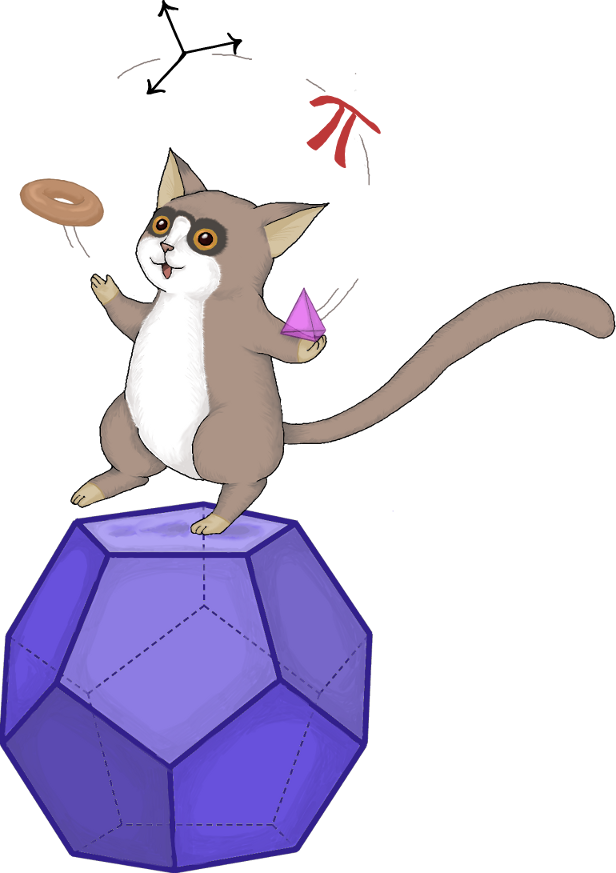
\includegraphics[scale=0.17]{cover}
}
\end{picture} 
	
\vspace{6em}

\begin{center}\Large{Mathe-Camp 2023}

\section*{Fraktale Dimensionen}\end{center}

\begin{defn}
	Wir sagen ein (geometrisches) Objekt hat \emph{Ähnlichkeitsdimension $d$} falls es eine Zahl $n \in \IN$ mit folgender Eigenschaft gibt:
	
	Strecken wir das Objekt um den Faktor $n$ (in alle Richtungen), so besteht das neue Objekt aus $n^d$ Kopien des ursprünglichen Objekts.
\end{defn}

Wir wollen uns zunächst überlegen, dass diese Dimensionsdefinition für viele \glqq normale\grqq{} Objekte mit unserer gewohnten Intuition für Dimension übereinstimmt:

\begin{aufg}
	Bestimme die Ähnlichkeitsdimension einer Strecke, eines Quadrats, eines Dreiecks, eines Würfels und eines Punktes. Du kannst dafür die folgende Tabelle benutzen:
	\begin{center}\renewcommand{\arraystretch}{2}
		\begin{tabular}{c||c|c|c|c||c}
			Streckfaktor: & \hspace{2em}2\hspace{2em} & \hspace{2em}3\hspace{2em} & \hspace{2em}4\hspace{2em} & \hspace{2em}9\hspace{2em} & Dimension\\\hline
			Linie & & & & & \\
			Quadrat & & & & & \\
			Dreieck & & & & & \\
			Würfel & & & & & \\
			Punkt & & & & & 
		\end{tabular}
	\end{center}
\end{aufg}

\section{Fraktale}

Betrachte das folgende Muster

\begin{center}
	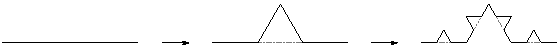
\includegraphics[width=.9\textwidth]{Bilder/Schneeflocke-Konstruktion1.pdf}
\end{center}

Kannst du dir vorstellen, was der nächste Schritt ist?

\begin{center}
	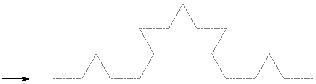
\includegraphics[width=.7\textwidth]{Bilder/Schneeflocke-Konstruktion2.pdf}
\end{center}

Und der nächste? Und...?

\begin{center}
	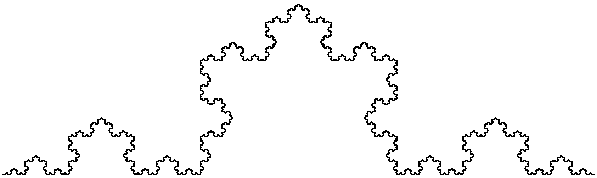
\includegraphics[width=.5\textwidth]{Bilder/Schneeflocke-Konstruktion3.pdf}
\end{center}

Das geometrische Objekt, das wir nach \emph{unendlich} vielen solcher Schritte erhalten, nennt man \emph{Kochsche Kurve}. Wir können das natürlich nicht wirklich zeichnen -- aber wenn wir die ersten Schritte auf dem Weg dorthin verstanden haben, können wir uns trotzdem ungefähr vorstellen, wie es aussehen sollte. Insbesondere können wir so auch mathematische Aussagen darüber treffen.

\begin{aufg}
	Bestimme die Ähnlichkeitsdimension der Kochschen Kurve. 
	
	\textit{Hinweis:} Es bietet sich dazu an die Kochsche Kurve um den Faktor $3$ oder $9$ zu strecken.
\end{aufg}

Die Kochsche Kurve ist ein Beispiel für ein sogenanntes Fraktal. Wir werden jetzt noch eine ganze Reihe weitere Fraktale kennenlernen:

\begin{itemize}
	\item Der \emph{Fraktal-Baum} ergibt sich durch folgenden Prozess:
		\begin{center}
			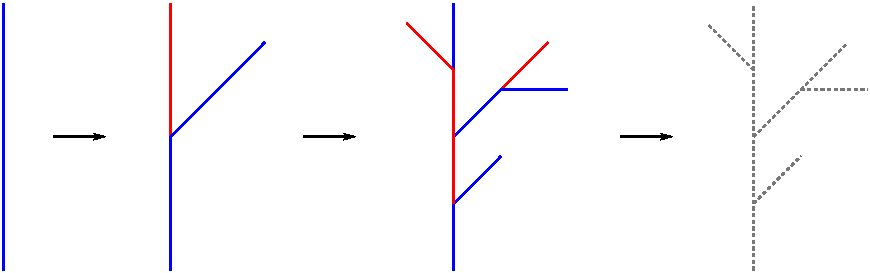
\includegraphics[width=.7\textwidth]{Bilder/Baum-Konstruktion.pdf}
		\end{center}
		Beachte, dass blaue und rote Linien jeweils einen leicht anderen nächsten Konstruktionsschritt haben.
		
	\item Die \emph{Drachenkurve} erhalten wir durch den folgenden Prozess
		\begin{center}
			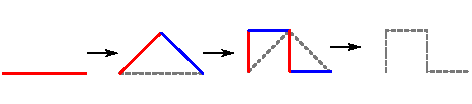
\includegraphics[width=.7\textwidth]{Bilder/Drachenkurve_Konstruktion.pdf}
		\end{center}
	
	\item Die \emph{Peano-Kurve} erhalten wir wie folgt:
		\begin{center}
			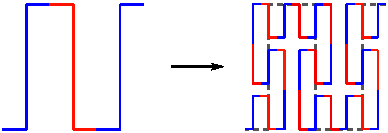
\includegraphics[width=.5\textwidth]{Bilder/Peano-Konstruktion.pdf}
		\end{center}
	
	\item Das \emph{Sierpinski-Dreieck} erhalten wir aus einem (ausgefüllten) gleichseitigen Dreieck, indem wir wiederholt kleinere gleichseitige Dreiecke ausschneiden:
		\begin{center}
			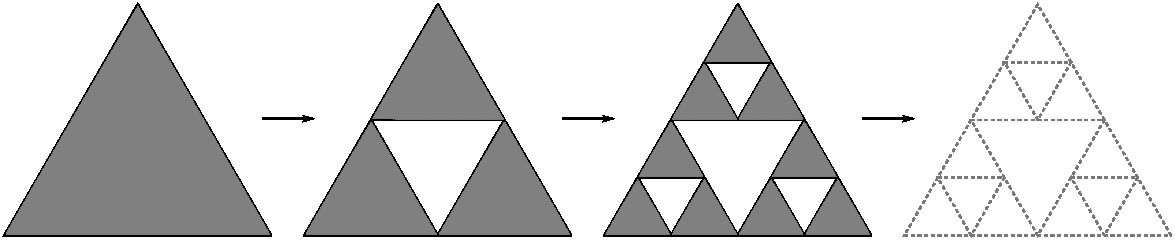
\includegraphics[width=.7\textwidth]{Bilder/Sierpinski-Konstruktion.pdf}
		\end{center}
	
	\item Analog erhalten wir die \emph{Sierpinski-Pyramide} aus einem (gefüllten) Tetraeder:
		\begin{center}
			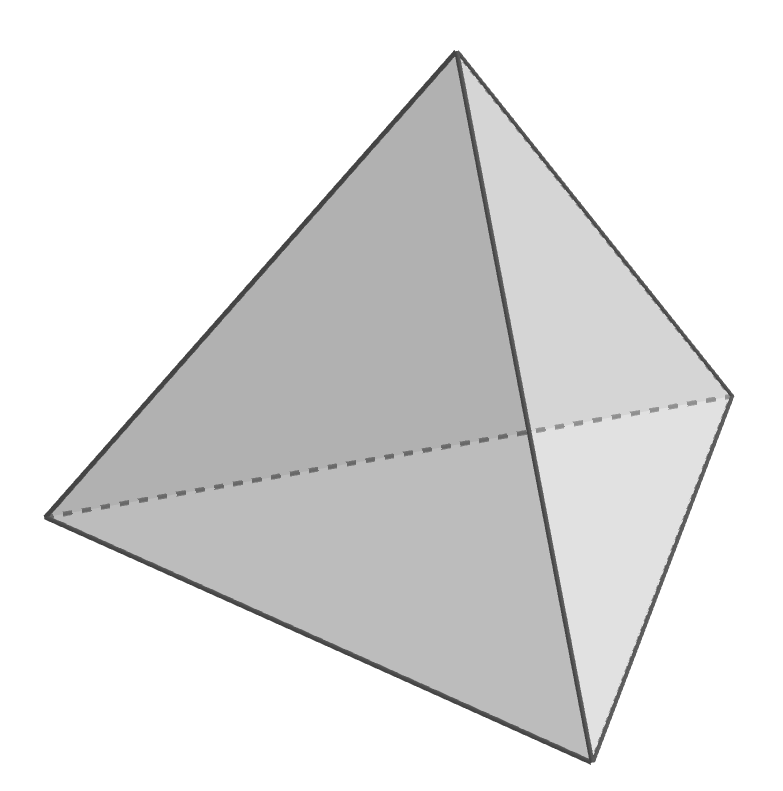
\includegraphics[width=.3\textwidth]{Bilder/Tetraeder.png} \hspace{3em} 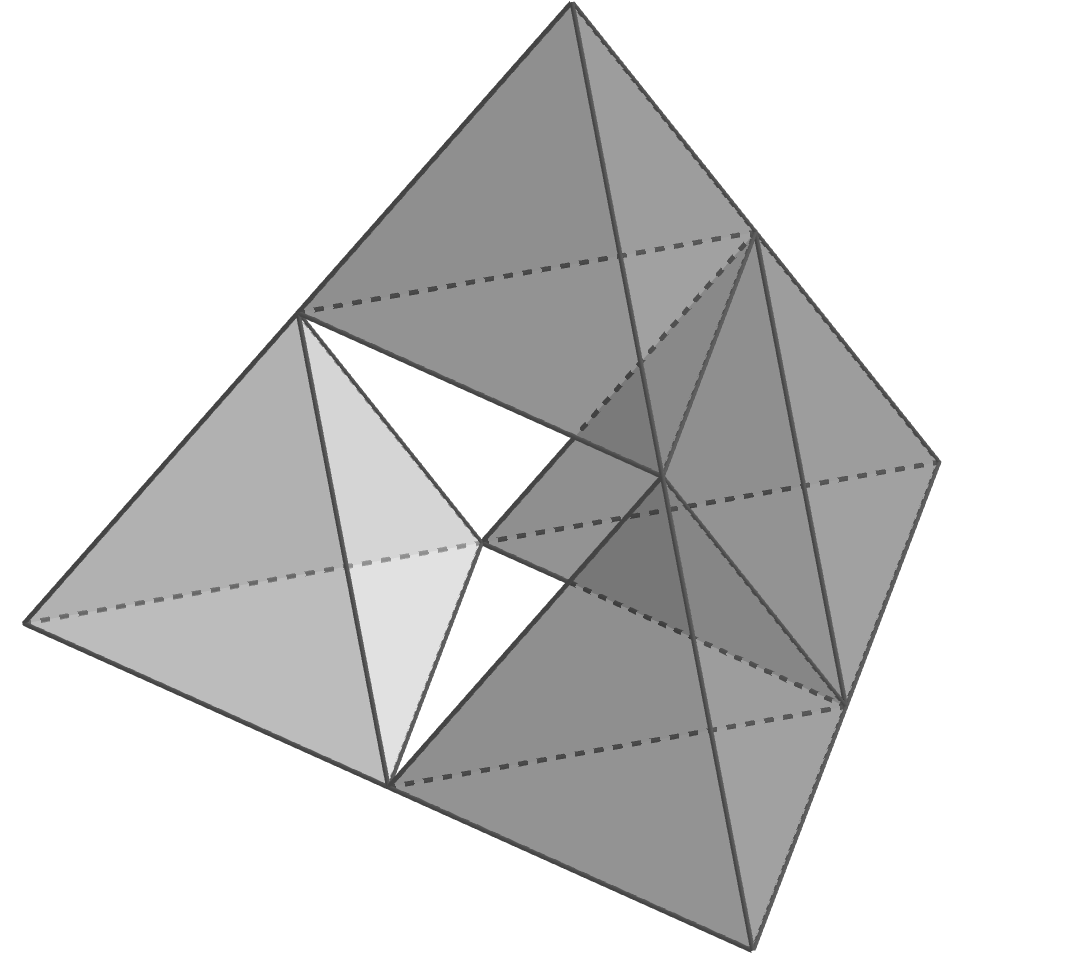
\includegraphics[width=.3\textwidth]{Bilder/Sierpinski-Pyramide.png}
		\end{center}

	\item Die \emph{Cantor-Menge} entsteht aus einer Strecke durch Ausschneiden des mittleren Drittels:
		\begin{center}
			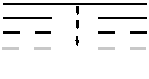
\includegraphics[width=.5\textwidth]{Bilder/Cantor_Menge.pdf}
		\end{center}
	
	\item Und es gibt noch viele mehr! Kannst du dir vielleicht sogar selbst ein Fraktal ausdenken?	
\end{itemize}

\begin{aufg}
	Bestimme die Ähnlichkeitsdimensionen dieser Fraktale.
\end{aufg}

\begin{bem}
	Angenommen wir untersuchen ein geometrisches Objekt und wollen dessen Dimension bestimmen. Wir haben es also um den Faktor $n$ gestreckt und festgestellt, dass das ursprüngliche Objekt nun $k$-mal in das neue hineinpasst. Wie können wir jetzt herausfinden, was die Dimension ist? Wie finden wir also ein $d$ mit $n^d = k$?
	
	Dazu gibt es die sogenannte \emph{Logarithmusfunktion} $\log_{\boxed{}}\boxed{\phantom{k}}$: Für zwei Zahlen $n$ und $k$ ist $\log_n k$ gerade die Zahl mit der wir $n$ potenzieren müssen um $k$ zu erhalten - d.h. $n^{\log_n k} = k$. Also ist $\log_n k$ gerade die Zahl, die auch unser $d$ sein soll. Wenn du einen Taschenrechner mit einer entsprechenden Funktion hast, kannst du das ja mal testen, indem du die fraktale Dimension der Kochschen Kurve nachrechnest.\footnote{Manche Taschenrechner haben keine allgemeine Logarithmus-Funktion, sondern nur eine, bei der du kein $n$ (sondern nur das $k$) angeben kannst. Dann kannst du dir mit folgender Rechenregel behelfen: $\log_n k = \frac{\log k}{\log n}$}
	
	Wenn du gerade keinen solchen Taschenrechner zur Hand hast, genügt es für das weitere Blatt aber auch, eine grobe Schätzung für $d$ zu finden. Zum Beispiel haben wir ja bereits herausgefunden, dass bei der Kochschen Kurve gilt: $3^d=4$ (in eine um den Faktor $3$ gestreckte Kochsche Kruve passt die ursprüngliche $4$-mal hinein). Jetzt können wir abschätzen:
	\[3^1 = 3 < 4 = 3^d = 4 < 9 = 3^2\]
	Also muss die fraktale Dimension der Kochschen Kurve irgendwo zwischen $1$ und $2$ liegen.
\end{bem}

\section{Wie groß ist ein Fraktal?}

Stell dir nun vor wir möchten eines der Fraktale schön bunt anmalen. Zum Beispiel würden wir gerne die Fläche unter der Kochschen Kurve ausmalen und dann auch ihren Rand farbig nachzeichnen. Was meinst du: Wie viel Farbe brauchen wir dafür jeweils?

\begin{lemma}
	Die Fläche unter der Kochschen Kurve ist endlich. Die Länge der Kochschen Kurve aber ist unendlich.
\end{lemma}

Dass die Fläche endlich ist, können wir beweisen, indem wir ein Objekt mit endlicher Fläche finden, in dem die Kochsche Kurve sicher enthalten ist. Um zu zeigen, dass die Länge unendlich ist, untersuchen wir, was mit der Länge in jedem einzelnen Schritt der Konstruktion passiert und überlegen uns dann, was nach unendlich vielen Schritten passiert ist.

\begin{aufg}
	Bestimme Länge/Fläche/Volumen der anderen Fraktale. Siehst du einen Zusammenhang zur Dimension dieser Fraktale?
\end{aufg}


\section{Woher kommen Fraktale?}

Fraktale tauchen in ganz verschiedenen Orten auf. Wir wollen hier drei solche kennenlernen:

\begin{itemize}
	\item Schneide einen Streifen Papier aus und falte diesen in der Mitte. Falte das Ergebnis erneut in der Mitte und so weiter (immer in die gleiche Richtung!)

	Wenn du nicht mehr weiter falten kannst, falte alles wieder auf, aber lasse alle Faltlinien zur Hälfte gefaltet (also $90^\circ$). Welches Fraktal siehst du?
	
	\item Kennst du das Pascalsche Dreieck? Befülle die folgend Figur so mit Zahlen, dass das Pascalsche Dreieck entsteht (in jedem der Sechsecke soll also eine Zahl stehen, wobei die Sechsecke am linken und rechten Rand $1$en enthalten und alle anderen Sechsecke die Summe der beiden Sechsecke direkt über diesem):
		
		\begin{center}
				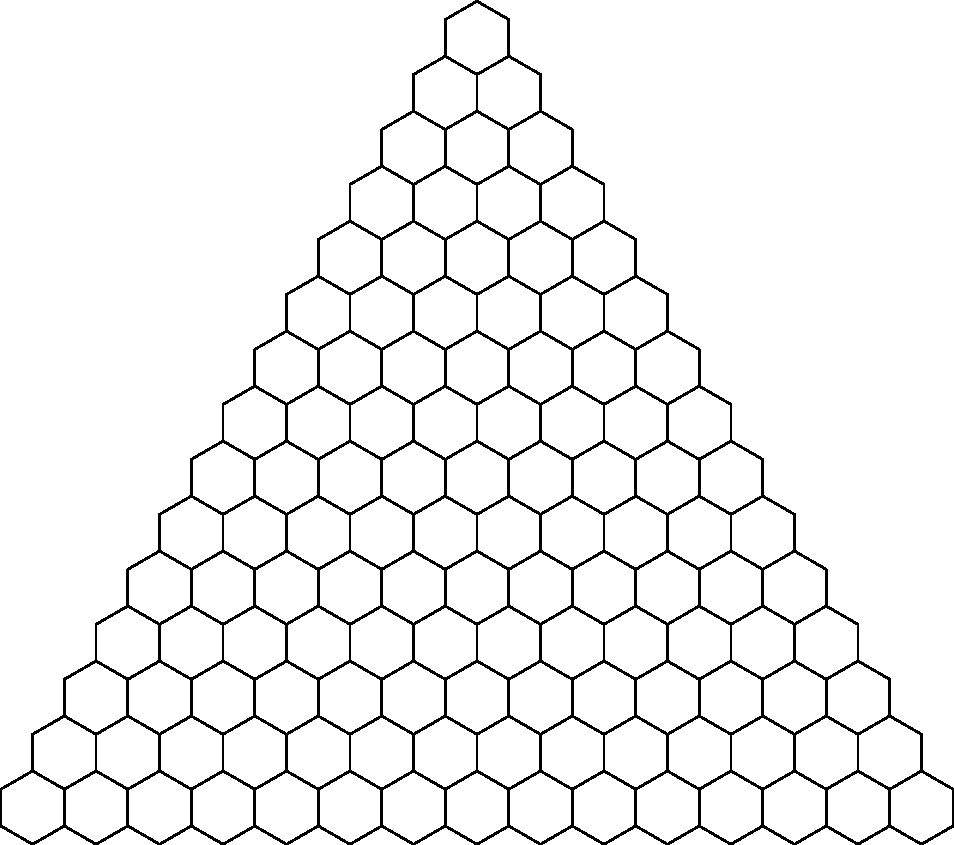
\includegraphics[width=.9\textwidth]{Bilder/Pascalsches-Dreieck.pdf}
		\end{center}
	
		Wenn du das gemacht hast, male alle Sechsecke aus, in denen eine ungerade Zahl steht. Fällt dir dabei etwas auf?
		
	\item Fraktale oder zumindest fraktalartige Dinge treten auch in der Natur auf. Und eines der häufigsten Beispiele dafür sind Meeresküsten -- wie zum Beispiel die deutsche Ostsee-Küste -- die du hier in drei verschiedenen Maßstäben abgebildet siehst:
	
	\begin{center}
		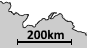
\includegraphics[width=.25\textwidth]{Bilder/Ostsee1.png}
		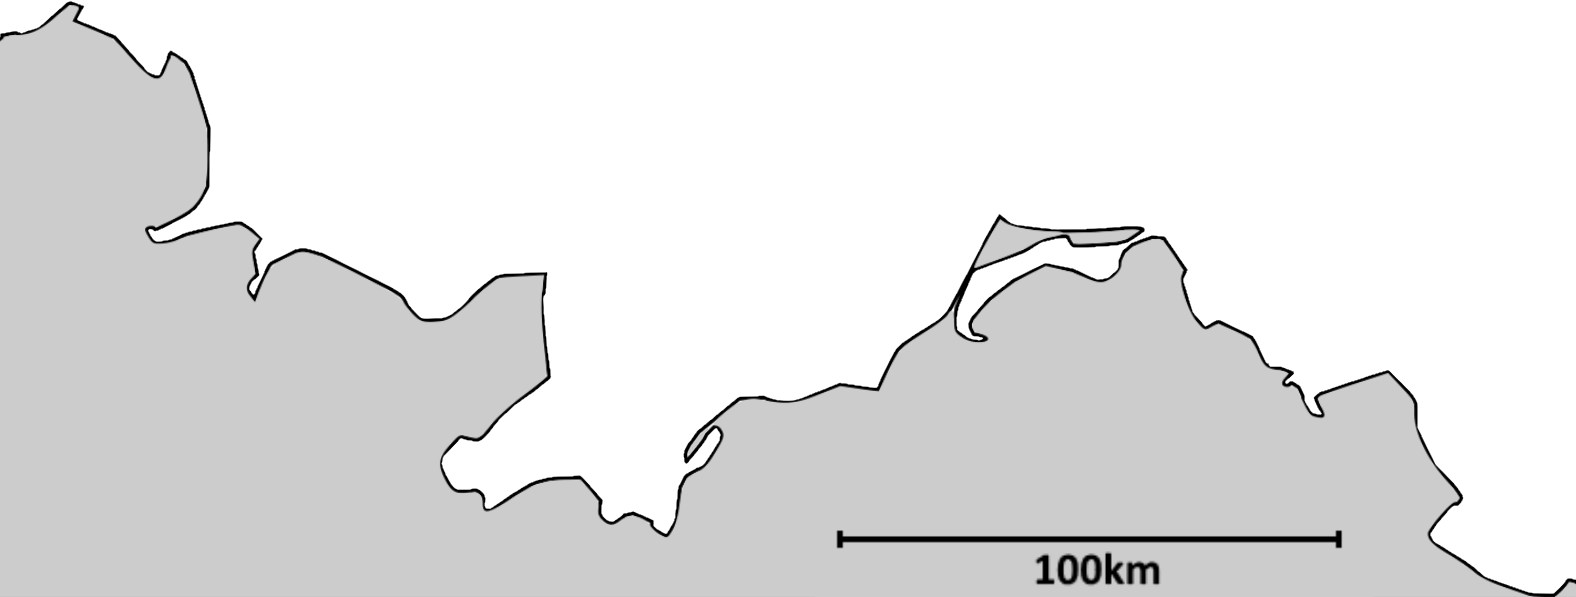
\includegraphics[width=.65\textwidth]{Bilder/Ostsee2.png}
		
		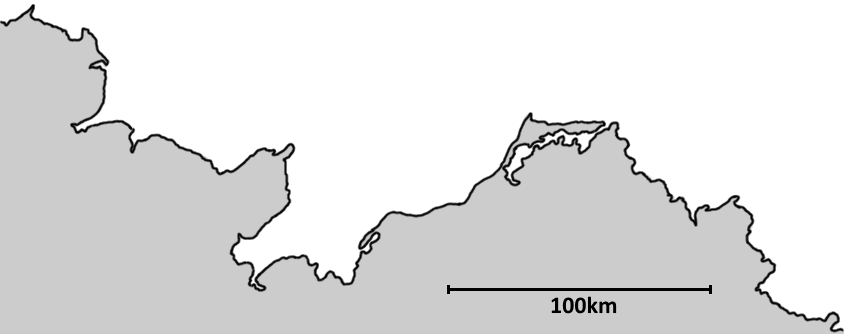
\includegraphics[width=.9\textwidth]{Bilder/Ostsee3.png}
	\end{center}

	Wenn du dir die obigen Bilder anschaust, kannst du vielleicht schon eine erste Ähnlichkeit zu unseren bisherigen Fraktalen erkennen: Je näher man an die Küstenlinie heranzoomt, desto mehr Zacken und Einbuchtungen kann man erkennen (so wie zum Beispiel auch bei der Kochschen Kurve). Gleichzeitig siehst du aber vermutlich auch, dass diese Küstenlinie nicht mit Hilfe einer so einfachen Konstruktionsvorschrift gezeichnet werden kann, wie das bei den bisherigen Fraktalen der Fall war.
	
	Daher können wir auch nicht so leicht die fraktale Dimension bestimmen wie das bisher der Fall war.\footnote{Es geht trotzdem - dafür bräuchten wir aber eine etwas andere Definition von Dimension.} Zumindest aber können wir versuchen ungefähr abzuschätzen, was die fraktale Dimension der Küstenlinie sein sollte -- insbesondere also, ob sie eine ganze Zahl ist oder nicht.
	
	Dafür werden wir gleich versuchen die Länge der Küstenlinie zu messen. Bevor du das machst, versuche folgende Fragen zu beantworten: Aufgrund deiner bisherigen Erfahrungen mit Fraktalen: Welche Länge sollte die Küste haben, wenn sie eine Dimension kleiner als $1$ hat? Welche Länge, wenn sie eine Dimension größer als $1$ hat? Und was wäre, wenn sie genau Dimension $1$ hätte (also überhaupt kein echtes Fraktal wäre)?
	
	Um die Länge der Küste zu messen, wollen wir wie folgt vorgehen: Zunächst wollen wir nur ganz grob die Länge bestimmen - dazu messen wir die Länge in der Karte mit dem größten Maßstab. Dann die im nächstgrößeren Maßstab. Und schließlich die im größten Maßstab. Trage deine Ergebnisse in der folgenden Tabelle ein (beachte, dass du die gemessenen Längen natürlich noch mit Hilfe des angegebenen Maßstabs in die tatsächlichen Längen umrechnen musst):
	
	\begin{center}
		\renewcommand{\arraystretch}{2}
		\begin{tabular}{l||c}
			& Länge der Küste in \unit{km} \\\hline\hline
			aus Karte 1 & \\\hline
			aus Karte 2 & \\\hline
			aus Karte 3 &
		\end{tabular}
	\end{center}
	
	Kannst du in der Tabelle ein Muster erkennen? Angenommen dieses Muster setzt sich auch bei weiteren, immer genaueren Messungen so fort - was würde dann wohl die tatsächliche Länge der deutschen Küste sein? Was kannst du damit über deren fraktale Dimension aussagen?
\end{itemize}

\end{document}